%================================================================
\section{Results}\label{sec:results}
% Present results and give a critical discussion of my work in 
% the context of other work. Relate the work to previous studies, 
% and make sure the results are reproducible. Include information 
% in figure captions such that they can give the reader enough to 
% understand the main gist of the report.
%================================================================

\subsection{Gradient descent}

We applied the gradient descent algorithm to data simulated from a third-degree polynomial without noise to assess convergence to the true parameters. All parameters converged after approximately 800 iterations using plain gradient descent (figure \ref{fig:poly-converge}). Adding momentum to the gradient descent sped up convergence to around 4-fold (figure \ref{fig:poly-converge-momentum}), and using any optimizer had similar effects on convergence times.

\begin{figure}
    \centering
    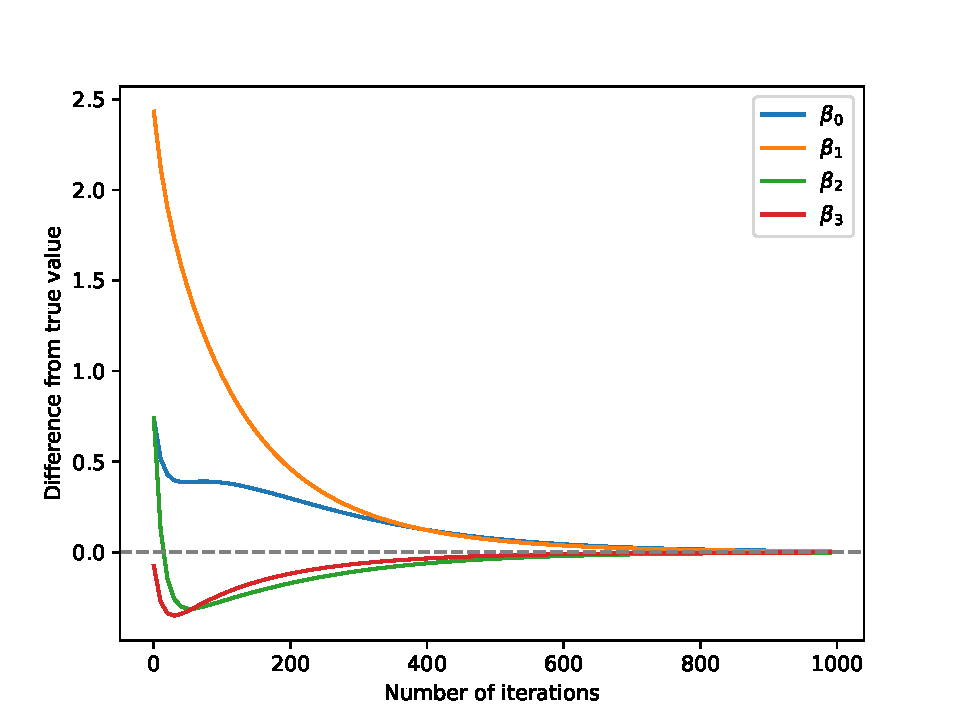
\includegraphics[width=0.99\linewidth]{examples/tests_even/figs/gradient-descent-polynomial-convergence.pdf}
    \caption{Gradient descent on data generated from a 4th degree polynomial without noise, using polynomial features up to the 4th degree. The stippled line represents 0 difference from the parameters used to generate the data.}
    \label{fig:poly-converge}
\end{figure}

\begin{figure}
    \centering
    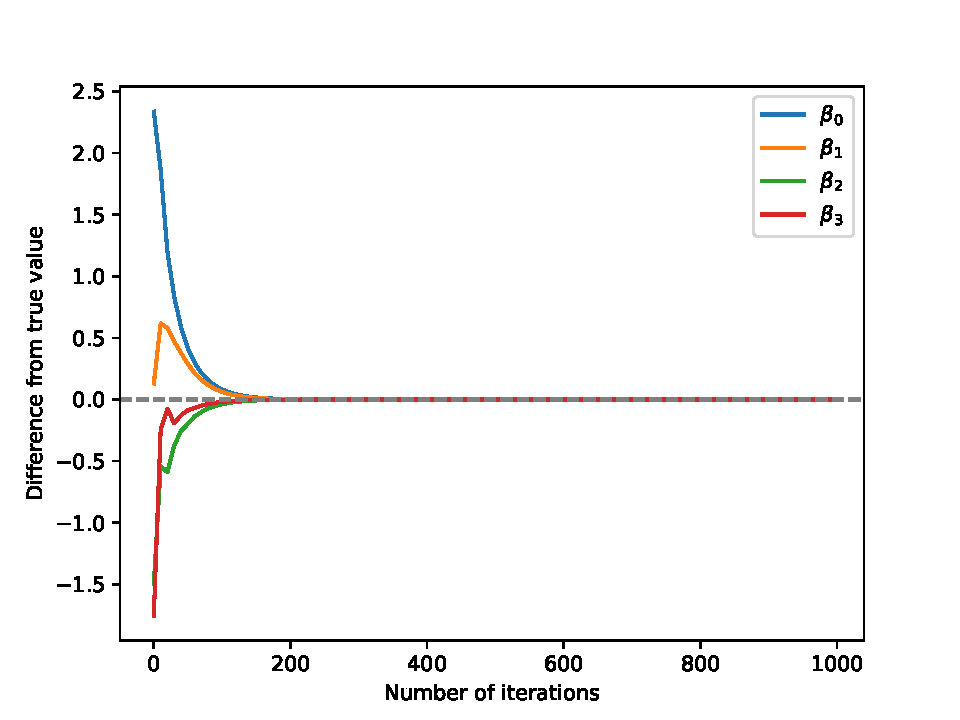
\includegraphics[width=0.99\linewidth]{examples/tests_even/figs/gradient-descent-momentum-polynomial-convergence.pdf}
    \caption{Gradient descent on the same data as in Figure \ref{fig:poly-converge}, but using momentum. The algorithm converged considerably faster than gradient descent without momentum.}
    \label{fig:poly-converge-momentum}
\end{figure}

We used simple data generated from the Franke function \cite{franke1979} with added noise to investigate the impact of learning rates and optimizers on gradient descent performance. The different optimizers had different optimal learning rates, but in general a learning rate between $10^{-3}$ and $1$ gave the best results (figure \ref{fig:franke-learningrate}). For this particular data GD outperformed SGD. Overall, ADAM consistently gave the lowest mean squared error on the test data over the largest range of learning rates. Because of this, we chose to emphasize ADAM over the other optimizers when analyzing the terrain data.

\begin{figure}
    \centering
    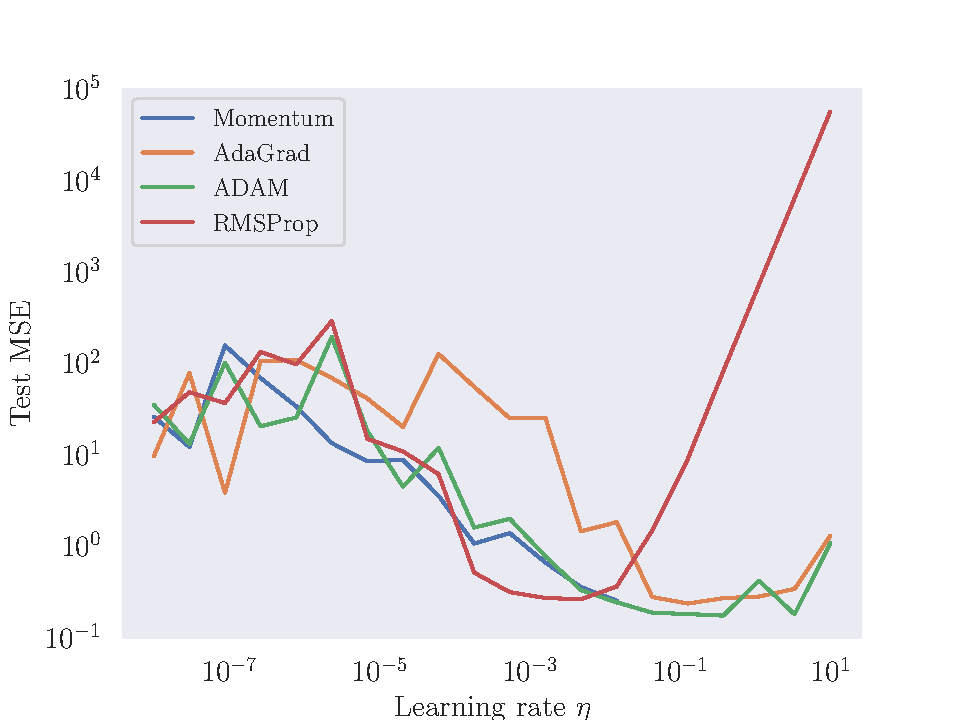
\includegraphics[width=0.99\linewidth]{examples/tests_even/figs/Franke-learningrates-optimizers.pdf}
    \caption{How learning rates affect the mean squared error in gradient descent with momentum or different optimizers. The data was generated from the Franke function, with added noise. For the momentum algorithm the gradient descent was not completed for learning rates above $10^{-2}$ due to exploding gradients.}
    \label{fig:franke-learningrate}
\end{figure}

We found the optimal parameters for gradient descent on the terrain data through a grid-search of $\lambda$ and learning rates. The optimal model was SGD with the ADAM optimizer, $\lambda=1.7\cdot10^{-6}$, and learning rate $\eta=1.78\cdot10^{-3}$, giving a test MSE of 0.19 on scaled, centered data. The model captured the general patterns in the terrain, but the predictions were less detailed than those from Ridge regression (Figure \ref{fig:terrain-allfigs}). This result is expected, as gradient descent with a Ridge gradient and polynomial features simply tries to approximate the best solution, which is found analytically in Ridge regression.

\subsection{Regression analysis with the feed-forward neural network}



\begin{figure*}[t]
    \centering
    \begin{tabular}{cc}
        \begin{subfigure}[b]{0.37\textwidth}
            \centering
            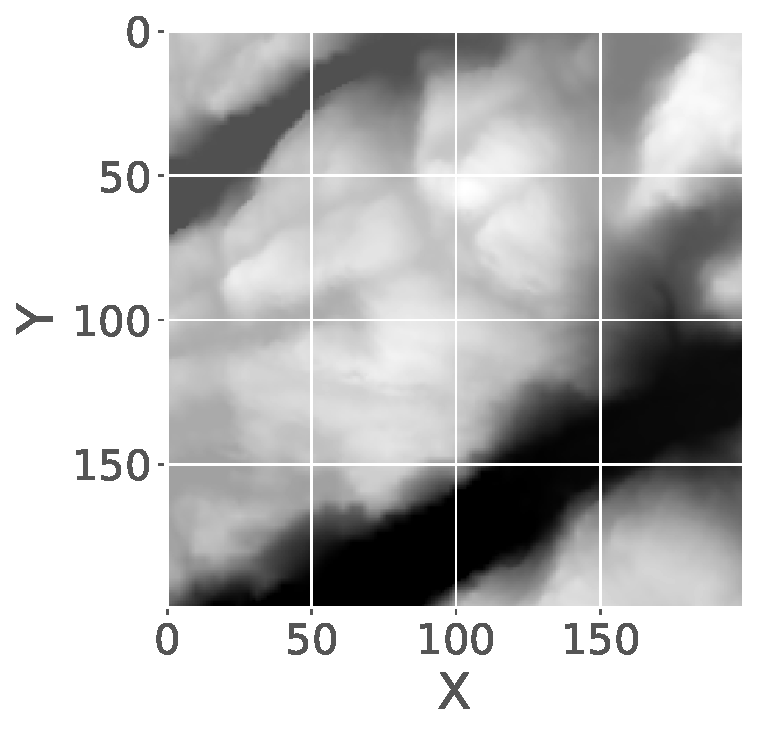
\includegraphics[width=\textwidth]{latex/figures/terrain1.pdf}
            \caption{Terrain}
            \label{fig:terrain1}
        \end{subfigure} &
        \begin{subfigure}[b]{0.37\textwidth}
            \centering
            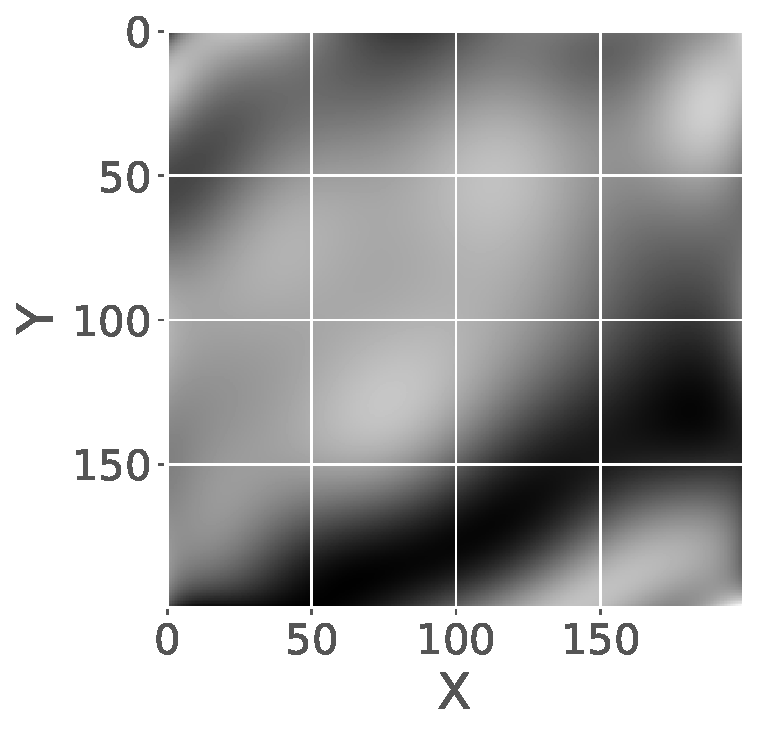
\includegraphics[width=\textwidth]{latex/figures/ridge_terrain1_prediction.pdf}
            \caption{Prediction from Ridge regression}
            \label{fig:terrain1-ridge}
        \end{subfigure} \\
        \begin{subfigure}[b]{0.5\textwidth}
            \centering
            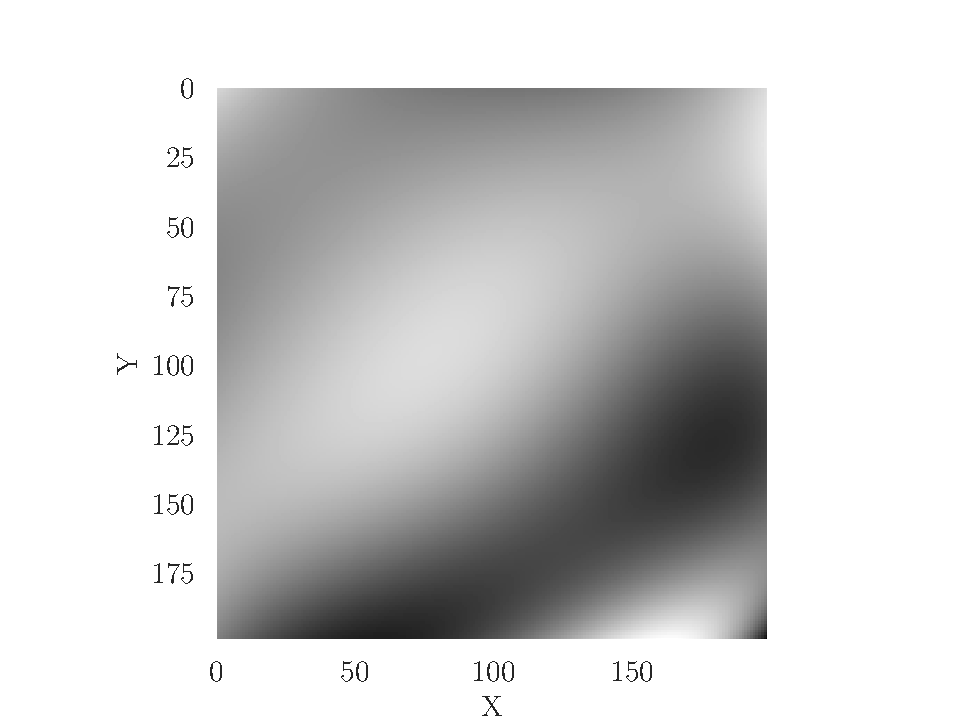
\includegraphics[width=\textwidth]{examples/tests_even/figs/gradient-descent-terrain-map.pdf}
            \caption{Prediction from stochastic gradient descent}
            \label{fig:terrain1-gd}
        \end{subfigure} &
        \begin{subfigure}[b]{0.5\textwidth}
            \centering
            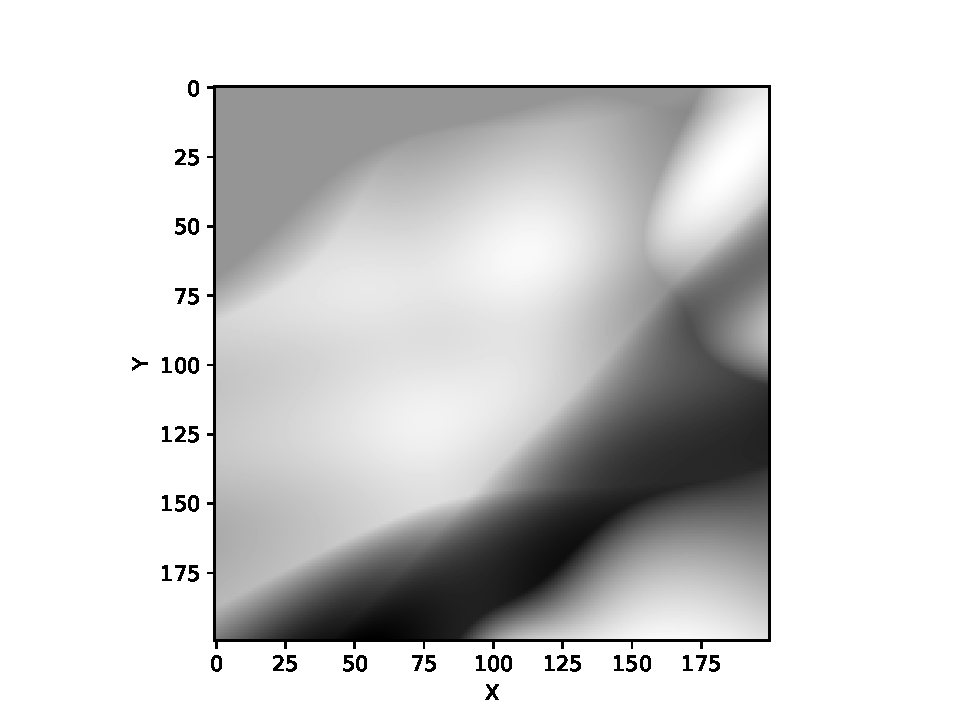
\includegraphics[width=\textwidth]{examples/tests_even/figs/neural-network-terrain-map.pdf}
            \caption{Prediction from the neural network}
            \label{fig:terrain1-nn}
        \end{subfigure}
    \end{tabular}
    \caption{Prediction of terrain data (a) using various methods.}
    \label{fig:terrain-allfigs}
\end{figure*}
\clearpage

- compare to project 1\\
- discuss results compared to OLS/Ridge\\
- Optimal learning rates and parameters, lambda-learningrate grid-search\\
- discuss activation functions\\
- discuss initialization of learning rates\\


\subsection{Breast cancer data}
We tested a set of different optimizers and learning rates on our breast cancer (BC) data, and found the best optimizer to be Adam, as is the golden standard for many NN problems today. The optimal learning rate with Adam was 0.1. To perform the classification we chose two layers of size 100 and 2, where our final layer output was a $n\ x\ 2$ vector with probabilities for each column, or diagnosis. We tested the network for up to 4 layers, but observed that accuracy on the test set decreased. This can be seen as a consequence of over-parametrization of the NN. Interestingly, the Sklearn NN acuracy fell more drastically that our NN, perhaps due to the 10-fold validatino step. For information about this selection process, see our appendix. "cite something?"

After splitting and normalizing the input data, we trained our neural net against Sklearns MLPClassifier with the same amount of layers. We chose the ReLU6 activation function for the first 100-node layer, and the final two-node layer had a sigmoidal activation function. For argumentation, see Subsection \ref{sssec:activation_functions}.

To prevent potential unwelcome batch effects that can occur from random splitting of test and train data, we did a 10-fold cross validation while training the NN and chose the back-propagation path with the best accuracy when testing on validation data. The result was suprisingly that our neural network performed better than Sklearn to a very small degree, as presented in Figure \ref{fig:our confusion matrix} and \ref{fig:sklearns confusion matrix}, as well as in \ref{fig:roc}.

\begin{figure}
    \centering
    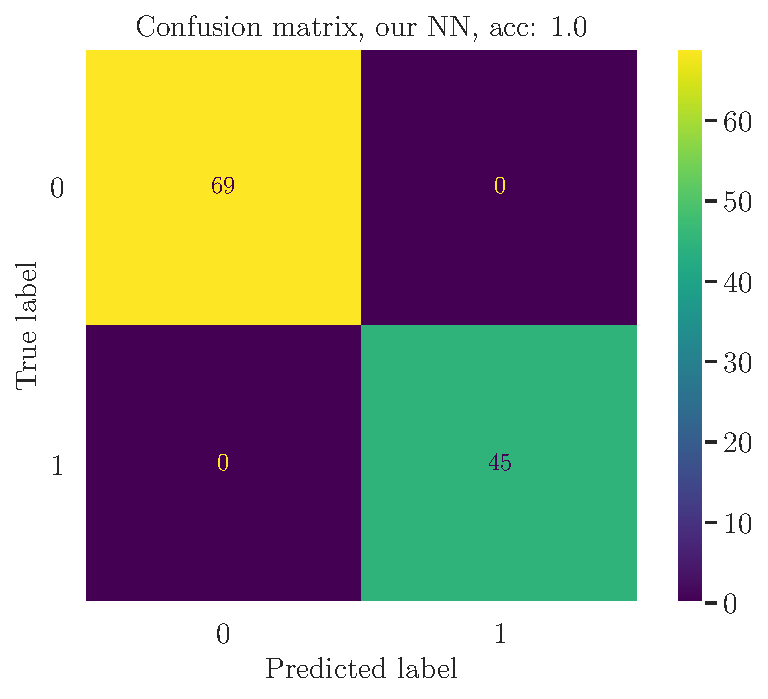
\includegraphics[width=0.99\linewidth]{figures/ourWBC_final_ADAM_relu6-100_sigmoid-2.pdf}
    \caption{Confusion matrix displaying how our NN performs on test data after training for 200 epochs with 10-fold cross validation. Accuracy of 1, as seen in plot title.}
    \label{fig:our confusion matrix}
\end{figure}

We then compared the same train and test set with the same amount of layers with Sklearn's classifier, which had a ReLU activation function and a sigmoidal activation function for the 100-node and 2-node layer, respectively. The results are presented in Figure \ref{fig:sklearns confusion matrix}. We summarize the sensitivity and specificity of both models in Table \ref{table:sensitivity-and-specificity}. Although our NN outperforms Sklearn's model in these results, we noticed that the final accuracy can vary, and their performance was quite similar on average based on our observations. 

\begin{figure}
    \centering
    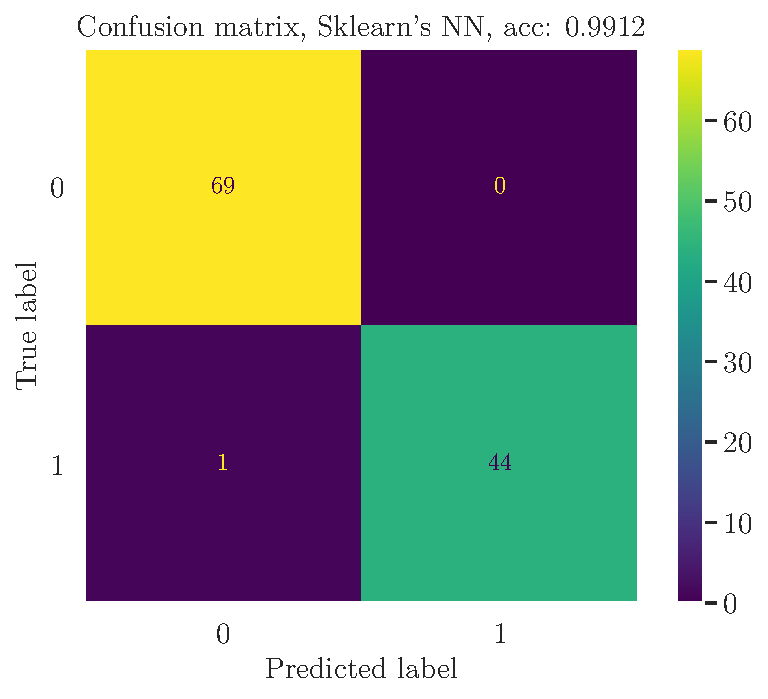
\includegraphics[width=0.99\linewidth]{latex/figures/sklearnWBC_final_ADAM_relu6-100_sigmoid-2.pdf}
    \caption{Confusion matrix displaying how Sklearn's NN performs on test data after training for 200 epochs. Accuracy of 0.9912, as seen in plot title.}
    \label{fig:sklearns confusion matrix}
\end{figure}

\begin{table}[h!]
\centering
\begin{tabular}{ccc}
\hline
\textbf{Method} & \textbf{Sensitivity} & \textbf{Specificity} \\
\hline
Our NN          & 1.0                           & 1.0                  \\
Sklearn's NN    & 0.9778                        & 1.0                  \\
\hline
\end{tabular}
\caption{Sensitivity and Specificity for each method based on the confusion matrices.}
\label{table:sensitivity-and-specificity}
\end{table}

\begin{figure}
    \centering
    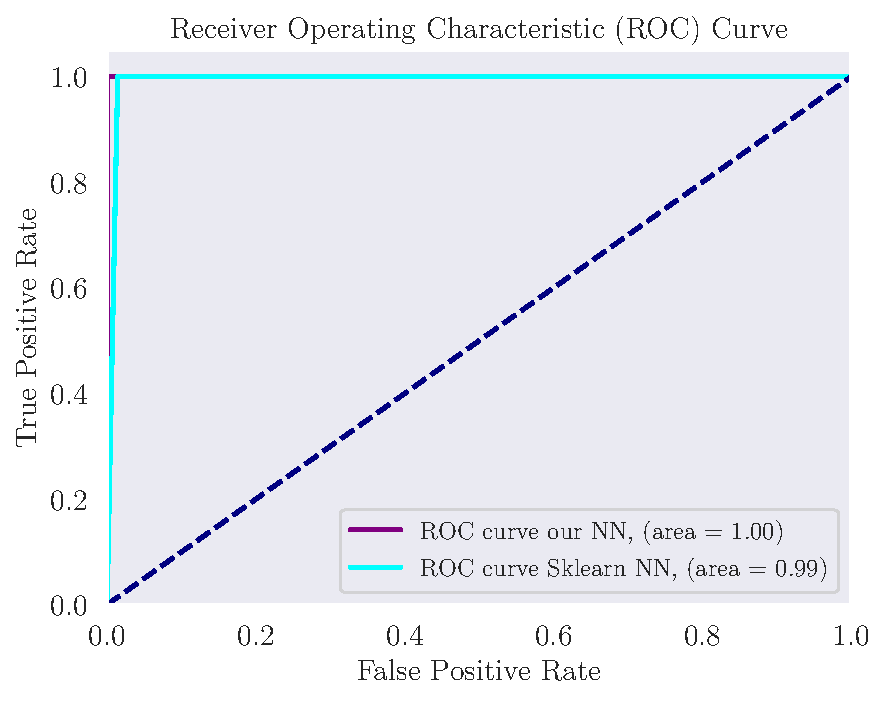
\includegraphics[width=0.99\linewidth]{latex/figures/ADAM_AUCROC_ADAM_relu6-100_sigmoid-2.pdf}
    \caption{Receiver operating characteristic (ROC) curve displaying the true positive rate against the false positive rate. The dotted line shows what our model would predict if outputs were completely random. The figure tells us that both models' predictions are perfect (our) or near perfect (Sklearn) predictors on the test data.}
    \label{fig:roc}
\end{figure}

- Compare with logistic regression\\

